%卒論概要テンプレート ver. 4.0

\documentclass[uplatex,twocolumn,dvipdfmx]{jsarticle}
\usepackage[top=22mm,bottom=22mm,left=22mm,right=22mm]{geometry}
\setlength{\columnsep}{11mm}
\usepackage[T1]{fontenc}
\usepackage{txfonts}
\usepackage[expert,deluxe]{otf}
\usepackage[dvipdfmx,hiresbb]{graphicx}
\usepackage[dvipdfmx]{hyperref}
\usepackage{pxjahyper}
\usepackage{secdot}





%タイトルと学生番号,名前だけ編集すること
\title{\vspace{-5mm}\fontsize{14pt}{0pt}\selectfont ディープラーニングを用いたWebサイトデザインの年代解析}
\author{\normalsize プロジェクトマネジメントコース 矢吹研究室 1442104 増田準}
\date{}
\pagestyle{empty}
\begin{document}
\fontsize{10.5pt}{\baselineskip}\selectfont
\maketitle





%以下が本文
\section{序論}\label{序論}

Webサイトのデザインは,時代に合ったものが求められる\cite{bib001}.スマートフォンの爆発的な普及により,Webサイトは急速に発展を遂げた.Webサイトをデザインするということは,視覚的な良し悪しを求めるだけでなく使いやすさなど様々な要素を含む.その為Webサイトを閲覧するデバイスによってデザインを変える事もあり,現代におけるWebデザインの多様化は著しい.更に,人々の生活に密接に影響していることから,Webサイトに対する研究は学際的に取り組まれている\cite{bib002}.以上のことから,本研究では時代によって進化するWebデザインの解析を対象とする.

\section{目的}

この研究は,年代ごとのWebデザインの変化を解析することが目的である.デザインとは数値などで表すことができるものではなく,漠然としたものである場合が多い.その為,解析の際はページに映る要素を総合的に判断させることが重要だ.

\section{手法}

この研究は以下の手法を用いて行う. 

\subsection{画像解析}

機械学習による画像解析を利用する.この研究における画像解析とは,多数の教師画像を学習させ判別モデルを作成し,別の画像を判別させることで画像の特徴を解析する処理を指す.

\subsection{画像の収集}

Internet Archiveにて閲覧できるWebページを,スクリーンショットを用いて多数保存する.対象となるWebサイトは2017年度版のFortune Global 500\cite{bib003}にリストされた企業のホームページとする. 


\section{結果}

上記した手法に乗っ取り,約14000枚の画像を取得した.その画像を使用し,数式処理ソフトMathematicaによる画像解析を行った.結果は次の図1の通りである.縦軸が算出された年代の値で,横軸が正解の値となっている.
\vspace{-1zh}
\begin{figure}[htb]
\centering
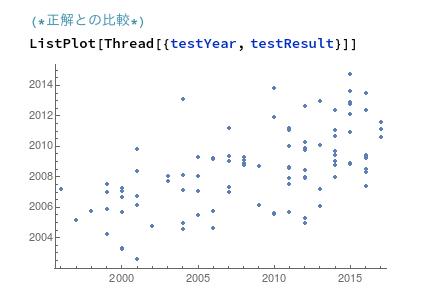
\includegraphics[width=6cm,clip]{graph.PNG}
\caption{Mathematicaによる
解析結果}
\end{figure}
\vspace{-1zh}

また,ディープラーニング用のツールNeural Network Consoleで画像解析した結果,正解率は40.75パーセントとなった.

\section{考察}

正解のばらつきが発生した原因は教師画像の不足していたことと,学習方法が最適でなかったことが考えられる.Mathematicaによる解析では,最終的に約14000枚で学習させたが,枚数を増やすごとにばらつきは少なくなった.また,Neural Network ConsoleではCNNの構築を最適化する機能によって同じ教師画像で正解率を上げることもできた.

\section{結論}

上記の結果と考察から,教師画像を更に増やし,CNNを最も適した形で構築し学習させることで,ディープラーニングによりWebデザインの年代を解析することは可能であると言える.

\bibliographystyle{junsrt}
\bibliography{biblio}%「biblio.bib」というファイルが必要.

\end{document}
